\section[Witnessing metrologically useful entanglement]
{Witnessing metrologically useful {\color{grey} X} entanglement}
\thiswatermark{\put(1,-282){\color{l-grey}\rule{84pt}{88pt}}
\put(84,-282){\color{grey}\rule{410pt}{88pt}}}


\quotes{Adrien-Marie Legendre}{All the truths of mathematics are linked to each other,

and all means of discovering them are equally admissible.}

\lettrine[lines=2, findent=3pt,nindent=0pt]{T}{ypically}, one has not access to the density matrix of the system been used for metrology or for other quantum process.
Moreover, for systems on which the particle number is very large, this is the case when one wants to do metrology with quantum states, the details of the density matrix are forbidden by practical reasons.
Since the quantum Fisher information is based on the complete knowledge of the density matrix, shortcuts to avoid the complete tomography must be developed as we have had shown one practical case on the previous chapter.
In this chapter, we obtain a general procedure to get an optimal bound for the quantum Fisher information based on as many expectation values of the initial state as one is ready to measure.
Two main features are worth to mention again.
First, in general this method gives us an optimal tight bound.
Last but not least, the bound is based on the expectation values of the initial state only, so it is not necessary to perform an evolution of the state to estimate how well will it behave.
This is in contrast to other approaches one can find in the literature, an it is a time saving concept.

The figure of merit of bounds from below for the quantum Fisher information based on expectation values of the initial state is the following,
\be
  \qfi [\rho,J_z] \geq \frac{\expect{J_x}^2}{\varian{J_y}}.
\ee
where the state is polarized along the $x$-axis and the variance of the $J_y$ operator is smaller than the standard.
On the previous chapter we also have shown one of these bound specifically designed for unpolarized Dicke states.

Homogeneous magnetometry, $\bs{B} = B\bs{k}$ where $B$ is constant in time.

Section~[REF], see magnetometry, generator $J_z$.

Quantum Fisher information $\qfi [\rho, J_z]$.

\subsection{Bound from below of a function convex over the states given some arbitrary expectation values}

The problem of getting a lower bound for a convex function on the states having already some expectation values of some arbitrary observables was studied by O. G\"uhne {\it et al.} and J. Eisert {\it et al.} in Refs.~\citep{Guehne2007, Eisert2007} respectively, mainly from the perspective of entanglement measures.
The illustrated techniques are based on the well known Legendre transform for differentiable functions, see Appedix~\ref{app:legendre-transform} for more details.
We first review in this section the state-of-the-art solution for this problem.
And later on, we extend it to the quantum Fisher information.
For simplicity in the next subsection, Sec~\ref{}, we assume that a single expectation value is given.
An extension to the case on which more expectation values are given will follow in the Subsection~\ref{}.
Finally, we will summarize it with an explicit formula which will be used to compute the bounds.

\subsubsection{Estimation of a general convex function based on the expectation value of an arbitrary observable}

When a convex function $g(\rho)$ is given together with an expectation value of some operator $w=\tr(\rho W)$, a tight lower bound, $\mathcal{B}_g(w)$, can be obtained as \citep{Rockafellar1996, Guehne2007, Eisert2007}
\be
  \label{eq:lt-lower-bound-single-parameter}
  \begin{split}
    g(\rho)\geq\mathcal{B}_g(w):=\,&\sup_r \{ rw - \hat{g}(rW)\}\\
    =\,& \{\inf_{\rho}g(\rho)\,|\,w = \tr(\rho W)\}
  \end{split}
\ee
where $\hat{g}(rW)$ is the Legendre transform of $g(\rho)$ and the second equality expresses the tightness of the bound.
The Legendre transform in this context is defined as
\be
  \label{eq:lt-for-convex-function-single-parameter}
  \hat{g}(rW)=\sup_{\rho}\{\expect{rW}_\rho - g(\rho)\},
\ee
where the maximisation is over \emph{all} possible states.
This method to obtain the lower bound has been used to compute entanglement measures, as we mentioned before [].

Following the theory one can find that in the case on which the convex function $g(\rho)$ is defined as convex roof over all possible convex decompositions of the state, the optimisation of Eq.~(\ref{eq:lt-for-convex-function-single-parameter}) can be reduced to an optimisation over pure states only, thus simplifying the process \cite{}
\be
\begin{split}
  \hat{g}(rW) & = \sup_{\rho}\{\expect{rW}_\rho - g(\rho)\} \\
  &=\sup_{\rho}\Big\{r\expect{W}_\rho - \inf_{\{p_k,\ket{\phi_k}\}}\big\{\sum_{k} p_k g(\ket{\phi_k})\big\} \Big\} \\
  &=\sup_{\{p_k, \ket{\phi_k}\}} \Big\{ \sum_k p_k \expect{rW}_{\ket{\phi_k}} - \inf_{\{p_k, \ket{\phi_k}\}} \big\{\sum_k p_k g(\ket{\phi_k}) \big\}  \Big\} \\
  &=\sup_{\{p_k, \ket{\phi_k}\}} \Big\{ \sum_k p_k \big\{ \expect{rW}_{\ket{\phi_k}} - g(\ket{\phi_k}) \big\} \Big\} \\
  &=\sup_{\ket{\psi}} \big\{ \expect{rW}_{\ket{\psi}} - g(\ket{\psi}) \big\}.
\end{split}
\ee
However, even an optimization over all pure states is feasible numerically only for small systems.
We will show later on this section how to circumvent this issue in the case of the QFI.
The convex roof construction has the following form
\be
  g(\rho) = \inf_{\{p_k,\psi_k\}} \sum_{k}p_k g(\ket{\psi_k}),
\ee
where the mixed state is decomposed into $\rho = \sum_k p_k \ketbra{\psi_k}{\psi_k}$.
Among other definitions of the QFI on the literature, there is one that defines it as the convex roof of $4\varian{J_z}$, the variance of the generator, as it has been shown on Ref.~\citep{Toth2007, }, we can compute the Legendre transform optimizing for pure states only.
Hence, we will be able to use this simplification to apply this method to obtain the lower bound on the QFI.
Notice that in this context the QFI is the convex roof of four times the variance of the generator, Eq.~\eqref{}.

\subsubsection{Measuring several observables}

For some cases, it is interesting to characterise the quantum state not only with a single measurement but with several.
For instance, we could want to use, as it is done with the spin-squeezed states the absolute polarisation and the variance of one of the orthogonal components of the angular momentum to detect entanglement and metrological usefulness \citep{}.
So far, we studied the case on which a single measurement is used.
Its extension to several expectation values is indeed straight-forward.
We can generalize Eqs.~\eqref{eq:lt-lower-bound-single-parameter} and \eqref{eq:lt-for-convex-function-single-parameter} for several observables $\{W_i\}_{i=1}^M$ as follows \citep{Guehne2007}
\be
  \label{eq:lt-extension-bound-multiparameter}.
  \mathcal{B}_g(w_1,w_2,\dots) := \sup_{\bs{r}}\big\{\bs{rw}-\sup_{\rho}\{\expect{\bs{rW}}-g(\rho)\}\big\},
\ee
where $\bs{ab} =\sum_{k=1}^M a_kb_k$, the usual notation for scalar products of two vectors.

\subsubsection{Explicit form of the expression to be optimized}

After we have shown how to find a lower bound for a general convex function of the state based on its expectation values and how to simplify that method for the case on which the function is defined as convex roof, now we are in a position to achieve the main goal of this chapter.
First of all, we notice that for the quantum Fisher Information the inner maximization, the Legendre transform, is obtained optimizing a quadratic function on expectation values,
\be
\label{eq:lt-legendre-of-qfi}
\begin{split}
  \hat{\qfi}(rW) &= \sup_{\ket{\psi}}\big\{r\expect{W}_{\psi}-4\varian{J_z}_{\psi}\big\} \\
  &= \sup_{\ket{\psi}} \big\{ r\expect{W}_{\psi}-4\expect{J_z^2}_{\psi} + 4\expect{J_z}^2_{\psi} \big\} \\
  &= \sup_{\ket{\psi}} \big\{\expect{rW-4J_z^2}_{\psi} +
  \expect{2J_z}^2_{\psi}\big\},
\end{split}
\ee
where we have used the fact that the QFI can be expressed as convex roof of $\varian{J_z}$ and we again fall into the problem of a single parameter for simplicity on the following derivations.
Equation~\eqref{eq:lt-legendre-of-qfi} can be rewritten as an optimization linear in operator expectation values and over a parameter $\mu$ as
\be
  \hat{\mathcal{F}}_{\text{Q}}(rW) = \sup_{\ket{\psi},\mu}\big\{\expect{rW-4J_z^2}_{\psi}+8\mu\expect{J_z}_\psi - 4 \mu^2\mtxid\big\},
\ee
which, making use of $\max\{\expect{A}\}=\lambda_{\max}[A]$ for any observable, can be reformulated as
\be
  \label{eq:lt-legendre-for-qfi-simplified}
  \begin{split}
    \hat{\mathcal{F}}_{\text{Q}}(rW) & = \sup_{\ket{\psi}}\big\{\lambda_{\max}[rW-4J_z^2+8\mu J_z - 4 \mu^2]\big\}\\
    &=\sup_{\ket{\psi}}\big\{\lambda_{\max}[rW-4(J_z-\mu)^2]\big\}
  \end{split}
\ee
where we omitted in writing $\mtxid$ for clarity and $\lambda_{\max}[A]$ stands for the maximum eigenvalue of the operator $A$.
At the extremum, we make the following observation, the derivative with respect to $\mu$ must be zero, hence at the optimum $\mu=\expect{J_z}_{\text{opt}}$ which represents the expectation value $J_z$ should have considering the optimal state on Eq.~\eqref{eq:lt-legendre-of-qfi}.
This also means that we have to test $\mu$ values in the interval $-N/2\leq\mu\leq N/2$ only for spin-half systems.

The full optimization problem to be solved consists of Eqs.~\eqref{eq:lt-lower-bound-single-parameter} and~\eqref{eq:lt-legendre-for-qfi-simplified} substituting $g(\rho)$ by $\qfi[\rho,J_z]$,
\be
  \mathcal{B}_{\mathcal{F}}(w) = \sup_r\big\{rw-\sup_{\mu}\{\lambda_{\max}[rW-4(J_z-\mu)^2]\}\big\}.
\ee
It is crucial that the optimization over $r$ is a concave function, since the theory tells us that $\hat{\mathcal{F}}_{\text{Q}}(rW)$ is a convex function \citep{}, even when the multi-parametric case is considered.
Thus the optimum can be determined easily with simple methods, e.g., the gradient method, looking for the maximum in $r$.
Based on Eq.~\eqref{eq:lt-lower-bound-single-parameter}, we can see that even if we do not find the global optimum in $r$, we obtain a valid lower bound.
The extension of this bound to the multi-parametric case is done using the recipie given in Eq.~\eqref{eq:lt-extension-bound-multiparameter}.
On the other hand, the function to be optimized for $\mu$ does not have a single maximum in general.
Moreover, not finding the optimal $\mu$ leads to an overestimating of the bound.
Thus, a large care must be taken especilly when optimizing over $\mu$.

We stress again the generality of this findings beyond linear interferometers covered on the following sections.
For nonlinear interferometers \citep{,,,,,}, the phase $\theta$ must be estimate in an unitary dynamics $U=\exp{-iG\theta}$, where $G$ is not a sum of single spin operators, hence, is different from the angular momentum components.

Next, we will demonstrate the use of our approach for several experimentally relevant situations.
In the many-particle case, often symmetric operators can be used to describe accurately the system, which makes possible to carry out calculations for thousand of particles, as will be presented later on this chapter.

\subsection{Examples}
\label{sec:lt-examples}

In this section, we show how to obtain lower bounds based of the fidelities with respect to the GHZ state and the unpolarized Dicke state as well as with different configurations of powers of collective angular momentum operators, e.g., the set $\{\expect{J_y}, \expect{J_x}, \expect{J_x^2}\}$.

\subsubsection{Exploiting symeetries}

When making calculations for quantum systems with an increasing number of qubits, we soon run into difficulties when computing the largest eigenvalue of Eq.~\eqref{eq:lt-legendre-for-qfi-simplified}.
The reason is that for $N$ qubits, we need to handle $2^N \times 2^N$ size matrices, hence we are limited to systems of 10 to 15 qubits.

We can obtain bounds for much larger particle numbers, if we restrict ourselves to the symmetric subspace \citep{}.
This approach can give optimal bounds for many systems, such as Bose-Einstein condensates (BEC) of two-level atoms, which are in a symmetric multiparticle state.
The bound computed for the syymmetric subspace might be not correct and generally overestimated for general cases.

Finally, it is important to note that if the operators $W_k$ are permutationally invariant and the eigenstate with the maximal eigenvalue in Eq.~\eqref{eq:lt-legendre-for-qfi-simplified} is non-degenerate.
And the resulting maximal eigenvalue is the same ...

We follow presenting the proof of the recently mentioned observation for completeness.
Let us denote the ground state of a permutationally invariant Hamiltonian by $\ket{\Psi}$
This is at the same time the $T=0$ thermal ground state, hence it must be a permutationally invariant pure state.
For such states $S_{kl}\ketbra{\Psi}{\Psi}S_{kl}=\ketbra{\Psi}{\Psi}$, where $S_{kl}$ is the swap operator exchanging qubits $k$ and $l$.
Based on this, follows that $S_{kl}\ket{\Psi}=c_{kl}\ket{\Psi}$, and $c_{kl}\in {-1,+1}$.
There are three possible cases to consider:
\begin{enumerate}
  \item All $c_{kl}=+1$.
  In this case, for all permutation operator $\Pi_j$ we have
  \be
    \label{eq:lt-permutating-ground-state}
    \Pi_j \ket{\Psi} = \ket{\Psi},
  \ee
  since any permutation operator $\Pi_j$ can be constructed as $\Pi_j=\prod_i S_{k_il_i}$.
  Equation~\eqref{eq:lt-permutating-ground-state} means that the state $\ket{\Psi}$ is symmetric.
  \item All $c_{kl}=-1$.
  This means that the state is antisymmetris, however this state exists only for $N=2$ qubits.
  \item Not all $c_{kl}$ are identical to each other.
  In this case, there must be $k_+,l_+,k_-,k_-$ such that
  \be
    \label{eq:lt-different-index-pi}
    \begin{split}
      S_{k_+,l_+} \ket{\Psi} & = +\ket{\Psi},\\
      S_{k_-,l_-} \ket{\Psi} & = -\ket{\Psi}.
    \end{split}
  \ee
  Let us assume that $k_+,l_+,k_-,l_-$ are index different from each other.
  In this case, $\ket{\Psi'}=S_{k_+,k_-}S_{l_+,l_-}\ket{\Psi}$ another ground state of the Hamiltonian $H$ such that
  \be
    \label{eq:lt-different-index-pi-2}
    \begin{split}
      S_{k_+,l_+} \ket{\Psi'} & = -\ket{\Psi'},\\
      S_{k_-,l_-} \ket{\Psi'} & = +\ket{\Psi'}.
    \end{split}
  \ee
  Comparing Eqs.~\eqref{eq:lt-different-index-pi} and \eqref{eq:lt-different-index-pi-2} we can conclude that $\ket{\Psi'}\neq\ket{\Psi}$, while due to the permutational invariance of $H$ we have that $\expect{H}_{\Psi'} = \expect{H}_{\Psi}$.
  Thus, $\ket{\Psi}$ is not a non-degenerate ground state.
  The proof works in an analogous way for the only nontrivial case $k_+=k_-$, when $S_{k_+,k_-}=\mtxid$.
\end{enumerate}

Hence, if $N>2$ then only i) is possible and $\ket{\Psi}$ must be symmetric.

\subsubsection{Fidelity measurements}

Let us consider the case when $W$ is a projector onto a pure quantum state.
First, we consider GHZ states \citep, hence $W$ is the projector $\ketbra{\ghz}{\ghz}$ and $\expect{W}=F_{\ghz}$, the fidelity with respect to the GHZ state.
Based on knowing $F_{\ghz}$, we would like to estimate $\qfi[\rho,J_z]$\footnote{Not a tight lower bounds on the quantum Fisher information based on the fidelity have been presented in \citep{}.}.

Using Eqs.~\eqref{} and \eqref{}, we will obtain an analytical tight lower bound on the QFI based on the fidelity $F_{\ghz}$. The calculation that we have to carry out is computing the bound
\be
  \label{eq:lt-maximization-problem-fid-ghz}
  \mathcal{B}_{\mathcal{F}}(F_{\ghz}) = \sup_r \big\{r F_{\ghz} - \sup_{\mu} \{\lambda_{\max}[r\ketbra{\ghz}{\ghz} - 4 (J_z - \mu)^2]\}\big\}.
\ee
We will make our calculations in the $J_z$ orthonormal basis, which is defined with the $2^N$ basis vectors $b_0= \ket{00\dots000}$, $b_1=\ket{00\dots001}$, \dots, $b_{(2^N-2)}=\ket{11\dots110}$, and $b_{(2^N-1)}=\ket{11\dots111}$.
It is easy to see that the matrix in the argument of $\lambda_{\max}$ in the Eq.~\eqref{eq:lt-maximization-problem-fid-ghz} is almost diagonal in the $J_z$ basis.
To be more specific, the only non-diagonal matrix block comes from $\ketbra{\ghz}{\ghz}$, which has non-trivial matrix elements only in the $\{b_0,b_{(2^N-1)}\}$ basis.
Thus, we have to diagonalize the following matrix
\be
  \label{eq:lt-expression-to-diagonalize-ghz}
  r\ketbra{\ghz}{\ghz} - 4 (J_z-\mu)^2 =
  \begin{pmatrix}
    \frac{r}{2}-4(\frac{N}{2}-\mu)^2 & \frac{r}{2}\\
    \frac{r}{2} & \frac{r}{2}-4(\frac{N}{2}+\mu)^2
  \end{pmatrix}
  \oplus D,
\ee
where $D$ is already a $(2^N-2)\times(2^N-2)$ diagonal matrix with $D_k=-4( \expect{J_z}_{b_k}-\mu)^2$ negative eigenvalues for $k=1,2,\dots, (2^N-2)$.
This means that the Eq.~\eqref{eq:lt-expression-to-diagonalize-ghz} can be diagonalized as $\text{diag}[\lambda_{+},\lambda_{-},D_1,D_2,\dots,D_{2^N-2}]$, where the two eigenvalues $\lambda_{\pm}$ are
\be
  \lambda_{\pm} = \frac{r}{2}-N^2-4 \mu^2\pm\sqrt{16\mu^2N^2+\frac{r^2}{4}}.
\ee

Next, we show a way that can simplify our calculations considerably.
As indicated in Eq.~\eqref{eq:lt-maximization-problem-fid-ghz}, we have to look for the maximal eigenvalue and then optimize it over $\mu$.
We exchange the order of the two steps, that is, we look for the maximum of each eigenvalue over $\mu$, and then find the maximal one.
Clearly based on the fact that the eigenvalues of $D$ are negative an that we can find a $\mu$ such that $D_k$ equal zero but not positive.
Due to this, the problem can be simplified to the following equation
\be
  \label{eq:lt-ghz-legendre-solution}
  \begin{split}
  \sup_{\mu}\{\lambda_{\max}[r\ketbra{\ghz}{\ghz}-4(J_z-\mu)^2]\}:= & \max\{0,\sup_{\mu}(\lambda_{+})\}\\
  = & \lcor
  \begin{aligned}
    &0, && \text{if } r<0,\\
    &\frac{r}{2}+\frac{r^2}{16N^2} && \text{if } 0\leq r\leq 4N^2,\\
    &-N^2+r, && \text{if }r>4N^2,
  \end{aligned}
  \right.
  \end{split}
\ee
where we did not have to have to look for the maximum of $\lambda_{-}$ over $\mu$ since clearly $\lambda_{+}\geq\lambda_{-}$.
Finally, we have to substitute Eq.~\eqref{eq:lt-ghz-legendre-solution} into Eq.~\eqref{eq:lt-maximization-problem-fid-ghz}, and carry out the optimization over $r$, considering $F_{\ghz}\in[0,1]$.

This way we arrive at the solution for the lower bound of the QFI base on the fidelity with respect to the GHZ state as
\be
  \mathcal{B}_{\mathcal{F}}(F_{\ghz}) = \lcor
  \begin{aligned}
    & N^2(1-F_{\ghz})^2, && \text{if } F_{\ghz} < 1/2, \\
    & 0, && \text{if } F_{\ghz}\leq1/2.
  \end{aligned}
  \right.
\ee
This equation is plotted in Figure~\ref{fig:lt-plots-for-fidelities}}~(a).
\begin{figure}
  \centering
  \igwithlabel{(a)}{scale=.65}{img/plots/LT_fidGHZ.pdf}
  \igwithlabel{(b)}{scale=.65}{img/plots/LT_fidDicke.pdf}
  \caption{(a) Analytical solution of the bound $\mathcal{B}_{\mathcal{F}}$ for different values of the fidelity with respect to the GHZ state. (b) Numerical results for the minimum quantum Fisher information as a function of the fidelity with respect of unpolarise Dicke states perpendicular to the magnetic field, $|\text{D}_N^0\rangle$. (blue-line) For systems with 4 particles and (red-dashed) for system with 8 particles. One may notice that when the fidelity is at its maximum the bound approaches to 0.5 as it is the quantum Fisher information for large particle number.}
  \label{fig:lt-plots-for-fidelities}
\end{figure}
Note that in the figure the plot is normalized by $N^2$ and that the resulting semi-parabola is independent of the number of particles.
Moreover, the bound is zero for $F_{\ghz}\leq 1/2$.
This is consistent with the fact that for the product states $\rho=\ket{111\dots11}$ or $\rho=\ket{000\dots00}$ we have $F_{\ghz}=1/2$, while $\mathcal{F}_{\text{Q}}[\rho,J_z]=0$.

Next, let us consider symmetric unpolarized Dicke state with even $N$ particles along the $x$-direction, which is given by
\be
  \label{eq:lt-unpolarized-z-dicke}
  \ket{\dicke{N,N/2}}_{x} =
  \begin{pmatrix}
    N\\
    N/2
  \end{pmatrix}^{-\frac{1}{2}} \sum_k \Pi_k (\ket{1}_{x}^{\otimes N/2}\ket{0}_{x}^{\otimes N/2}),
\ee
where the summation is over all the different permutations, $\Pi_k$, of the product state having $N/2$ particles in $\ket{1}_{x}$ and the rest $N/2$ in the $\ket{0}_{x}$ state, the single qubit $j_x^{(n)}$ basis states.

This state is known to be highly entangled \citep{,} and allows for Heisenberg limited interferometry \citep{}.
In the following we will omit the second subscript and we use the notation $\ket{\dicke{N}}_{x}\equiv \ket{\dicke{N,N/2}}_{x}$, where we even may skip the subscript $x$ since this Dicke state will be always in the center of our attention, the unpolarized Dicke state perpendicular to the magnetic field in this case along the $z$-direction.
The witness operator that can be used for noisy Dicke states is $W=\ketbra{D_N}{D_N}$, hence the expectation value of the witness is just the fidelity with respect to the Dicke state, i.e., $\expect{W}=F_{\text{Dicke}}$.
In Figure~\ref{fig:lt-plots-for-fidelities}~(b), we plotted the results for symmetric Dicke states of various spin numbers.
$F_{\text{Dicke}}=1$ corresponds to $\mathcal{F}_{\text{Q}}[\rho,J_z]=N(N+2)/2$.
At this point, note that for the examples presented above, the QFI bound scales as $\mathcal{O}(N^2)$ in the asymptotic limit if the quantum state has been prepared perfectly\footnote{$\mathcal{O}(x)$ is the usual Landau notation used to describe the asymptotic behavior for large $x$ \citep{,}.}.

Note that estimating $\qfi[\rho, J_z]$ based on $F_{\text{Dicke}}$ was possible for 40 qubits [TD: Ask geza for the data points for 40 particles] for Fig~\ref{fig:lt-plots-for-fidelities}~(b), since we carried out the calculations for the symmetric subspace.
For our case, the witness operator $W$ is permutationally invariant and it has a non-degenerate eigenstate corresponding to the maximal eigenvalue.
Hence, based on the arguments of the Section~\ref{sec:} the bound is valid even for general case, i.e., non-symmetric states.

We now compute several quantities for the large $N$ case.
We show that if the fidelity with respect to the Dicke state is larger than a bound then $\mathcal{B}_{\mathcal{F}}>0$.
Moreover, we have seen in Figure~\ref{fig:lt-plots-for-fidelities}~(b) that the lower bound on $\qfi[\rho,J_z]$ as a function of the fidelity $F_{\text{Dicke}}$ normalized by $N^2$ is not the same curve for all $N$.
Next, we will demonstrate by numerical evidence that the lower bound normalized by $N^2$ collapses to a nontrivial curve for large $N$.

As a first step, let us consider the completely polarized state along $z$-direction $\ket{1}_y^{\otimes N}$.
This state does not change under rotations around the $z$-axis, hence $\qfi[\rho,J_z]=0$.
Its fidelity with respect to the Dicke state, Eq.~\eqref{eq:lt-unpolarized-z-dicke}, is
\be
  \label{eq:lt-fidelity-dicke-with-tp}
  F_{\text{Dicke}}(\ket{1}_y^{\otimes N}) = \frac{1}{2^N}\binom{N}{N/2}\approx \sqrt{\frac{2}{\pi N}}
\ee
From convexity of the bound on the quantum Fisher information in $F_{\text{Dicke}}$, it immediately follows that for $F_{\text{Dicke}}$ smaller than Eq.~\eqref{eq:lt-fidelity-dicke-with-tp} the optimal bound on $\qfi[\rho,J_z]$ will give zero.

Next, we examine what happens if the fidelity is larger than Eq.~\eqref{eq:lt-fidelity-dicke-with-tp}.
For that we notice first that $\qfi[\rho,J_z]$ is the convex roof of $4\varian{J_z}$ \citep{}.
Hence, if we have a mixed state for which $\qfi[\rho,J_z]$ is zero, then it can always be decomposed into the mixture of pure states for which $\qfi[\ket{\Psi},J_z]$ is zero too.
As a consequence, the extremal states of the set of states for which $\qfi[\rho,J_z]=0$ are pure states, and we can restrict our search for pure states.
The optimization problem we have to solve is given as
\be
  F_{\text{opt}} = \big\{ \max_{\Psi} |\braket{\Psi}{\dicke{N}}_x|^2 \,|\, \qfi[\ket{\Psi},J_z]=0\big\}.
\ee
Pure states $\ket{\Psi}$ that are invariant under $U_{\theta}=\exp(-iJ_z\theta)$ for any $\theta$.
Such states are the eigenstates of $J_z$.
In order to maximize the overlap with the Dicke state $\ket{\dicke{N}}_{x}$, we have to look for symmetric eigenstates of $J_z$.
These are the symmetric Dicke states in the $z$-basis $\ket{\dicke{N,m}}_z$.
Then, using the following identity
\be
  \sum_{k=0}^q \binom{n}{k}\binom{n}{q-k}(-1)^k = \lcor
  \begin{aligned}
    &\binom{n}{q/2}(-1)^{q/2},&& \text{for even }q,\\
    &0, && \text{for odd }q.
  \end{aligned}
  \right.
\ee
one finds that the squared overlap is given by
\be
  \label{eq:lt-dicke-overlap-with-tp}
  |\braopket{\dicke{N,m}}{_z}{\dicke{N}}_x|^2 = \lcor
  \begin{aligned}
    &\frac{\binom{N/2}{m/2}^2\binom{N}{N/2}}{2^N\binom{N}{m}} ,&& \text{for even }m \text{ and }N,\\
    &0, && \text{for odd }m,
  \end{aligned}
  \right.
\ee
which maximal, in the case of even $N$, when $m=N$ or $m=0$, thus the totally or anti-totally polarized states respectively.
We skip the case on which $N$ is odd.
For detailed calculations of Eq.~\eqref{eq:lt-dicke-overlap-with-tp} see Appendix~\ref{app:calculation-dicke-overlap}.

Next, we will examine the behavior of our lower bound on $\qfi[\rho,J_z]$ based on the fidelity $F_{\text{Dicke}}$ for large $N$.
In figure~\ref{} [TD: Ask Geza for the data], the calculations up to $N=500$ present a strong evidence that for fidelity values $F_{\text{Dicke}}=0.2,0.5,0.8$ the lower bound on QFI has a $\mathcal{O}(N^2)$ scaling for increasing $N$.
If this is correct then reaching a fidelity larger than a certain monotonously decreasing bound for large $N$ would imply Heisenberg scaling for the bound on the quantum Fisher information.
Note that it is difficult to present a similar numerical evidence for small values of $F_{\text{Dicke}}$ since in that case the bound for QFI is nonzero only for large $N$ due to Eq.~\eqref{eq:lt-fidelity-dicke-with-tp}.

\subsubsection{Spin-squeezed states}

In the case of spin squeezing, the quantum state has a large spin in the $y$-direction, while a decreased variance in the $x$-direction.
By measuring $\expect{J_y}$ and $\varian{J_x}$ we can estimate the lower bound for the quantum Fisher Information by Eq.~\eqref{eq:lt-pezze-smerzi}.
However, this formula does not necessarily give the best lower bound for all values of the collective observables.
With our approach we can find the best bound.

To give a concrete example, we choose $W_1=J_y$, $W_2=J_x^2$ and $W_3=J_x$ for the operators to be measured.
We vary $w_1$ and $w_2$ in some interval.
We also require that $w_3=0$, since we assume that the mean spin points into the $y$-direction\footnote{Due to symmetries of the problem, when minimizing $\qfi[\rho,J_z]$ with the constraints on $\expect{J_z}$ and $\expect{J_x^2}$, we do not have to add explicitly the constraint $\expect{J_x}=0$.
Optimization with only the first two constraints will give the same bound (see Section~\ref{sec:}).}
This is reasonable since in most spin-squeezing experiments we know the direction of the mean spin.

Our result can be seen in Figure~\ref{fig:lt-spsq2d-4}.
\begin{figure}
  \centering
  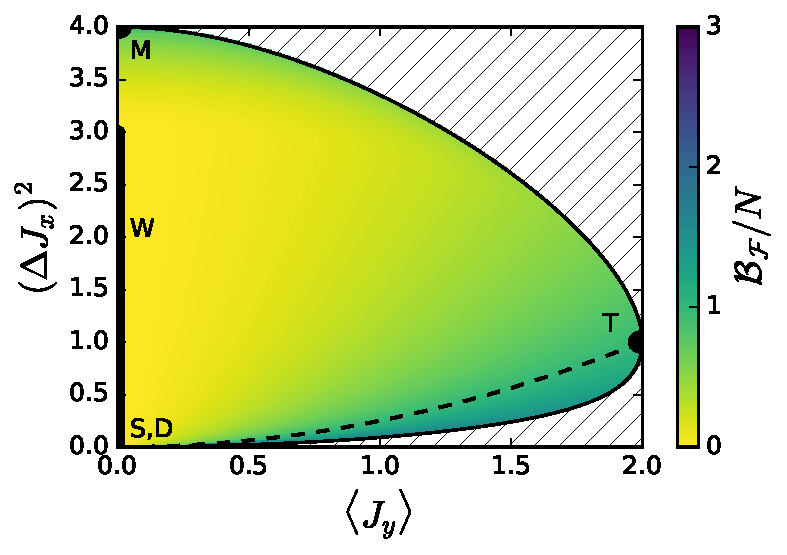
\includegraphics[scale=.65]{img/plots/LT_spsq2d_4.pdf}
  \caption{We show as a function of the expectation value, $\expect{J_y}$, and the variance in the perpendicular direction, $\varian{J_x}$, the minimum sensitivity for a 4-qubit system.
  (hatched) The physically forbidden region is indicated. (M,T,S,D) Those points indicate where the mixed state (), the totally polarized state (), the single state and the unpolarized Dicke state would be located. (W) on this line sit any of the states which is a mixture between the completely mixed state of the symmetric subspace and the singlet state among others, for instance the completely mixed state of the whole Hilbert space. (dashed) It indicates the shot-noise threshold where below it non-classical sensitivities can be achieved.}
  \label{fig:lt-spsq2d-4}
\end{figure}
We chose $N=4$ particles since for small $N$ the main features of the plot are clearly visible.
The hatched area correspond to non-physical conbination of expectation values.
States at the boundary can be obtained as ground states of $H_{\text{bnd}}^{(\pm)}(\lambda)=\pm J_x^2 -\lambda J_y$, see Appendix~\ref{app:spin-squeezing-hamiltonian}.
In Figure~\ref{fig:lt-spsq2d-4}, the state fully polarized in the $y$-direction, and initial state for spin-squeezing experiments, corresponds to point T.
The unpolarized Dicke state along $x$-direction Eq.~\eqref{eq:lt-unpolarized-z-dicke} corresponds to point D.
We add that outside the symmetric subspace, there are other states with $\expect{J_y}=\expect{J_x^2}=0$, which also corresponds to point D (in this case denoted by point S).
For example, such a state is the multiparticle singlet corresponding to point S.
However, usual spin-squeezing procedures remain in the symmetric subspace, thus we discuss only the Dicke state.
Spin squeezing makes $\varian{J_x}$ decrease, while $\expect{J_y}$ aslo decreased somewhat.
Hence, at least for small squeezing it corresponds moving down from point T to point D following the boundary, while the metrological usefulness is increasing.
Below the dashed line $\qfi[\rho,J_z]>N$, hence the state possesses metrologicaly useful entanglement \citep{}.
The equal mixture of $\ket{000\dots00}_x$ and $\ket{111\dots11}_x$ corresponds to point M, with $\qfi[\rho,J_z] = N$.
Finally, the completely mixed state rests on the line W.
It cannot be used for metrology, hence $\qfi[\rho,J_z]=0$.

We now compare the difference between our bound and L.~Pezze and A.~Smerzi bound Eq.~\eqref{eq:}.
First, we consider the experimentally relevant region for which $\varian{J_x}\leq 1$.
We find that for points away from the physical boundary at least by 0.001 on the vertical axis, the difference between the two bounds is smaller than $2\times10^{-6}$.
For points at the boundary, the difference is somewhat larger, but still small, the relative difference is smaller than $2\%$ for 4 particles.
[TD: Add part of the appendix]
Hence, Eq.~\eqref{eq:} practically coincides with the optimal bound for $\varian{J_x}<1$.

We now consider regions on Figure~\ref{fig:lt-spsq2d-4} for which $\varian{J_x}>1$.
The difference between the two bound is now larger.
It is larger at point M, for which the bound Eq.~\eqref{eq:} is zero.
Hence for measurement values corresponding to points close to M, our method improve the formula Eq.~\eqref{eq:}.
It is important from the point of view of applying our method to spin-squeezing experiments that the bound Eq.~\eqref{eq:} can be substantially improved for $\varian{J_x}<1$, if we assume bosonic symmetry for the system, or we measure an additional quantity, such as $\expect{J_x^4}$ as shown in Figure~\ref{fig:lt-} [TD: Ask Geza for data].

\begin{figure}
  \centering
  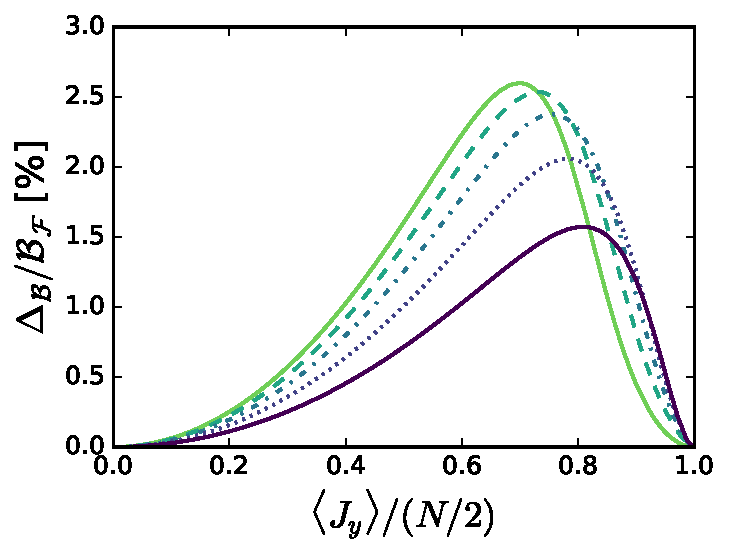
\includegraphics[scale=.65]{img/plots/LT_edge_diff.pdf}
  \caption{Difference between the bound of Pezze-Smerzi and the optimal bound for the quantum Fisher information normalized by the value of the optimal bound itself for the bosonic ground states of $H=J_x^2-\lambda J_y$ for $\forall \lambda \in [0,\infty)$.
  From dark to lighter colors (line, point, dash-point, dashed, pointed, line), results for different particle numbers, $N=4,6,10,20,1000$ respectively.
  Heuristically speaking, one can say that for large particle number the difference is biggest when the polarisation is around two thirds of the maximal polarisation and that this difference is about $2.6\%$.}
  \label{fig:lt-edge-diff}
\end{figure}

\subsubsection{Dicke states}
In this section, we use our method to find lower bounds on the QFI for states characterized to be close to the Dicke state \eqref{eq:lt-unpolarized-z-dicke}.

\begin{figure}
  \centering
  \igwithlabel{(a)}{scale=.65}{img/plots/LT_spsq_scaling_1.pdf}
  \igwithlabel{(b)}{scale=.65}{img/plots/LT_spsq_scaling_2.pdf}
  \caption{}
  \label{fig:lt-spsq-scaling}
\end{figure}

\begin{figure}
  \centering
  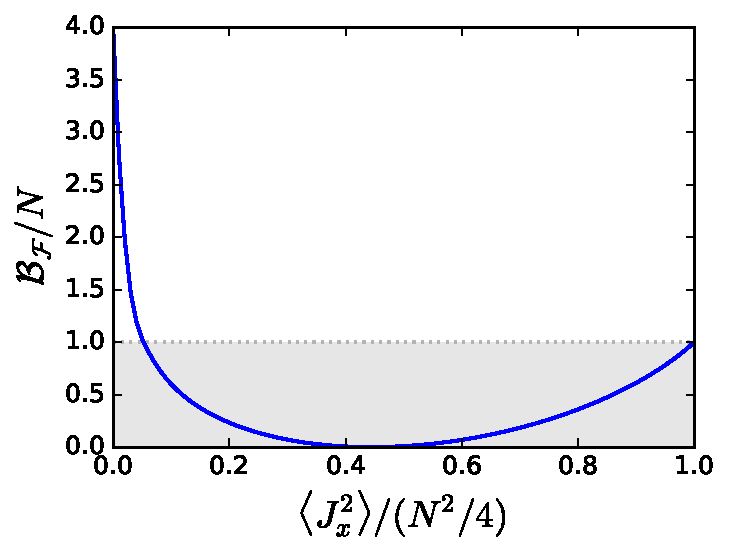
\includegraphics[scale=.65]{img/plots/LT_dicke_edge.pdf}
  \caption{The numerics shows us a tiny region the symmetric system surpassing the shot-noise threshold.}
  \label{fig:vd-secuence-evo}
\end{figure}

\begin{figure}
  \centering
  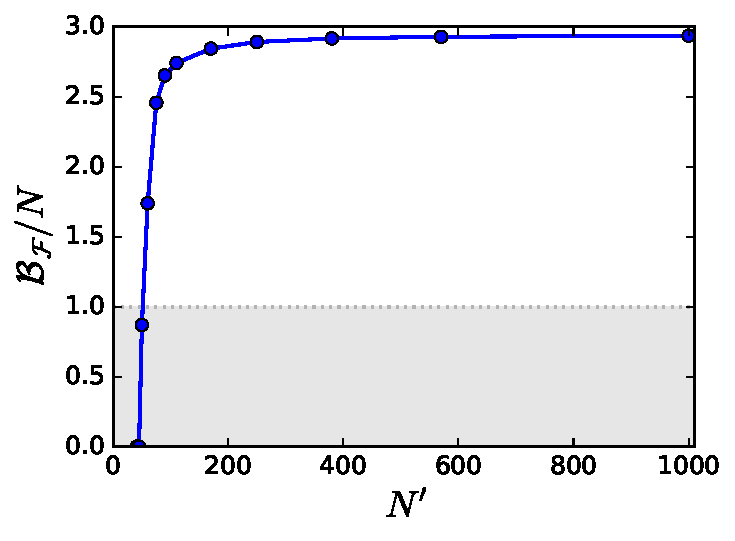
\includegraphics[scale=.65]{img/plots/LT_dicke_7900_asymp.pdf}
  \caption{Secuence of the evolution of an unpolarized Dicke state of 16 qubits for $\Theta=\{i\pi/6\}_{i=0}^4$. Bloch spheres representing the Hirusi distribution of the state, and below PDF of the $J_x$ POVM for each step of the secuence}
  \label{fig:vd-secuence-evo}
\end{figure}
